% ==============================================================================
% CHƯƠNG 3: CHUẨN BỊ DỮ LIỆU (DATA PREPARATION)
% ==============================================================================

\chapter{Chuẩn Bị Dữ Liệu và Kiến Trúc Medallion (Data Preparation)}
\label{chap:data_preparation}

\section{Chiến Lược Thu Thập Dữ Liệu 3 Tầng (Three-Tier Pipeline)}

Để vừa bắt kịp các công trình nghiên cứu mới công bố hàng ngày, vừa đảm bảo chiều sâu lịch sử cho mạng lưới trích dẫn, hệ thống xây dựng quy trình thu thập dữ liệu tự động gồm 3 tầng (Three-Tier Harvesting Architecture) được lập lịch và điều phối bởi \textbf{Apache Airflow 2.10} theo múi giờ chuẩn Việt Nam (\path{Asia/Ho_Chi_Minh - ICT}):

\begin{enumerate}[label=\textbf{\arabic*.}]
  \item \textbf{Tier 1: Real-Time Stream (Hàng ngày lúc 19:00 ICT)}:
    \begin{itemize}
      \item \textit{Nguồn \& Phương thức}: Quét tự động các RSS Feeds chính thức của arXiv trên 5 chuyên ngành: \texttt{cs.AI}, \texttt{cs.LG}, \texttt{cs.CV}, \texttt{cs.CL}, và \texttt{stat.ML}.
      \item \textit{Trách nhiệm}: Bắt kịp các ấn phẩm tiền công bố trong vòng 24 giờ qua. Các bản ghi thu thập được đẩy ngay lập tức vào hàng đợi thông điệp RabbitMQ (\texttt{scientific\_paper\_ingest}) để worker bóc tách và nhúng vector vào Qdrant, phục vụ các truy vấn thời sự của người dùng.
    \end{itemize}
  \item \textbf{Tier 2: Near-Past Harvest (Hàng ngày lúc 19:10 ICT)}:
    \begin{itemize}
      \item \textit{Nguồn \& Phương thức}: CVF (CVPR/ICCV/WACV và workshop) luân phiên với arXiv OAI-PMH, mỗi nguồn khoảng một giờ. arXiv đi ngược từng ngày đến 01/01/2024, dùng cursor và tuân thủ Retry-After khi bị giới hạn tốc độ.
      \item \textit{Trách nhiệm}: Thu thập trong ngân sách \texttt{LAKEHOUSE\_BUDGET\_GB}, mặc định 20 GB; không có chỉ tiêu cố định 10,000 bài. Mỗi lô tối đa 1,000 bản ghi, chờ hàng đợi ingest giảm dưới ngưỡng rồi tiếp tục, cân bằng nhóm ngành và nguồn.
    \end{itemize}
  \item \textbf{Tier 3: Historical Landmark Archive (Thủ công; DAG không đặt lịch)}:
    \begin{itemize}
      \item \textit{Nguồn \& Phương thức}: DAG landmark dùng Semantic Scholar và bổ sung metadata từ arXiv. OpenAlex/Zenodo là nguồn bổ trợ được đề cập trong thiết kế và các module khác, không phải cả ba đều được DAG landmark hiện tại gọi.
      \item \textit{Trách nhiệm}: Bổ sung công trình có ảnh hưởng và tài liệu lịch sử; mức độ trung tâm của từng bài cần được xác định từ artifact graph thực tế.
    \end{itemize}
\end{enumerate}

\section{Bóc Tách Văn Bản Học Thuật và Bảo Toàn Công Thức Toán}

Khác với các tài liệu văn phòng thông thường, tài liệu khoa học chứa đựng cấu trúc ngữ nghĩa chặt chẽ và hàm lượng phương trình toán học dày đặc. Module \texttt{AcademicHTMLParser} (triển khai tại \path{src/transformation/html_parser.py}) được thiết kế chuyên biệt để phân tích các tài liệu HTML5 học thuật:

\begin{enumerate}[label=\alph*)]
  \item \textbf{Nhận dạng và phân loại Section}: Áp dụng các biểu thức chính quy (Regular Expressions) để phân loại từng đề mục vào các loại chuẩn: \texttt{abstract}, \texttt{introduction}, \texttt{related\_work}, \texttt{methodology}, \texttt{experiments}, \texttt{discussion}, \texttt{conclusion}, và \texttt{appendix}.
  \item \textbf{Bảo toàn ký hiệu toán LaTeX}: Công cụ duyệt tìm các phần tử toán học dạng thẻ \texttt{<math>} hoặc \texttt{<span class="ltx\_Math">}, ưu tiên trích xuất chuỗi LaTeX gốc từ thẻ con \path{annotation encoding="application/x-tex"} hoặc thuộc tính \texttt{alttext}. Parser hiện đóng gói công thức nhận được trong \lstinline{$...$}; không có nhánh phân biệt display bằng \lstinline{$$...$$}. Khi thiếu annotation/alttext, parser dùng text hiển thị làm fallback, nên cần kiểm tra chất lượng công thức sau trích xuất.
  \item \textbf{Loại bỏ nhiễu và làm sạch cấu trúc}: Tự động loại bỏ các thẻ script, navigation bar, style, header/footer của trang web, chuẩn hóa các khoảng trắng thừa nhưng bảo tồn nguyên vẹn cấu trúc đoạn văn (\texttt{<p>}).
\end{enumerate}

\section{Chuẩn Hóa Dữ Liệu và Cơ Chế Toàn Vẹn SHA-256}
\begin{itemize}
\item \textbf{Định danh}: Mã arXiv được chuẩn hóa, bỏ URL và hậu tố phiên bản khi kiểm tra trùng.
\item \textbf{Khử trùng lặp}: Fetch kiểm tra \texttt{paper\_id} và \texttt{abstract\_hash} trong Silver. Hash được tạo bằng SHA-256 sau chuẩn hóa Unicode NFKC, chữ thường, loại HTML, dấu câu và gộp khoảng trắng; khi abstract trống, Silver writer dùng title. Compaction papers giữ bản ghi ghi sau cùng cho mỗi \texttt{paper\_id}.
\item \textbf{Toàn vẹn đối tượng}: Storage có tiện ích SHA-256 cho dữ liệu/file tải lên. Hash đối tượng phục vụ kiểm tra byte; \texttt{abstract\_hash} phục vụ dedup. Schema papers hiện không có \texttt{content\_hash} tính từ toàn văn.
\end{itemize}

\section{Kiến Trúc Hồ Dữ Liệu Medallion (Medallion Lakehouse)}

Hệ thống triển khai kiến trúc \textbf{Medallion Lakehouse} chuẩn công nghiệp, phân tách triệt để giữa tầng tính toán (Compute) và tầng lưu trữ (Storage) nhằm tối ưu hóa chi phí và khả năng mở rộng:

\begin{enumerate}[label=\textbf{\arabic*.}]
  \item \textbf{Bronze Zone (\path{s3://uth-scientific-lakehouse/bronze/papers/YYYY/})}:
    Lưu trữ nguyên bản các tệp JSON siêu dữ liệu thô và tệp HTML5 học thuật được cào từ arXiv/ar5iv. Dữ liệu tại tầng này mang tính bất biến (immutable), cho phép hệ thống tái xử lý từ đầu bất cứ khi nào cập nhật thuật toán bóc tách mới.
  \item \textbf{Silver Zone (\path{s3://uth-scientific-lakehouse/silver/papers/year=YYYY/})}:
    Dữ liệu sau khi làm sạch được chuyển đổi sang định dạng cột \textbf{Apache Parquet}, nén bằng thuật toán \texttt{zstd} (Zstandard) mức nén tối ưu. Dữ liệu được phân vùng (partitioned) theo năm xuất bản. Tại tầng này, công cụ \textbf{DuckDB OLAP} có thể truy vấn trực tiếp dữ liệu từ S3 với kỹ thuật \textit{Predicate Pushdown} và \textit{Column Projection}, giảm dữ liệu cần đọc; thời gian thực tế phụ thuộc số part, dung lượng và mạng.
  \item \textbf{Silver chunks (\path{silver/chunks/year=YYYY/})}: Một dòng cho mỗi chunk, gồm ID, title, authors, text, section và \texttt{indexed\_at}. Embed ghi part trước khi upsert vector. Compaction tạo \texttt{chunks.parquet}, giữ lần indexing mới nhất theo bài; lookup ưu tiên bản mới nhất theo chunk ID và chỉ đọc row group cần thiết.
  \item \textbf{Gold Zone}:
    \begin{itemize}
      \item \textit{Vector Store (Qdrant)}: Lưu trữ các vector biểu diễn ngữ nghĩa 768 chiều của các đoạn văn bản học thuật (\texttt{scientific\_papers\_gold}) được chỉ mục bằng đồ thị HNSW (Hierarchical Navigable Small World) viết bằng Rust, hỗ trợ lọc theo metadata. Payload chỉ gồm \texttt{chunk\_id}, \texttt{paper\_id}, \texttt{year}, \texttt{primary\_category}, \texttt{section\_type}; nội dung được hydrate từ Silver chunks. Metadata năm lấy từ ngày công bố khi có.
      \item \textit{Mining Artifacts (\path{s3://.../gold/mining/})}: Lưu trữ các tệp JSON tri thức cô đọng được xuất ra từ 4 Trụ cột Khai phá: đồ thị mạng lưới \path{graph_coauthorship.json}, tập luật kết hợp \path{association_rules.json}, phân cụm \texttt{clusters.json}, và danh sách dị biệt \path{trends_anomalies.json}.
    \end{itemize}
\end{enumerate}

\begin{figure}[htbp]
  \centering
  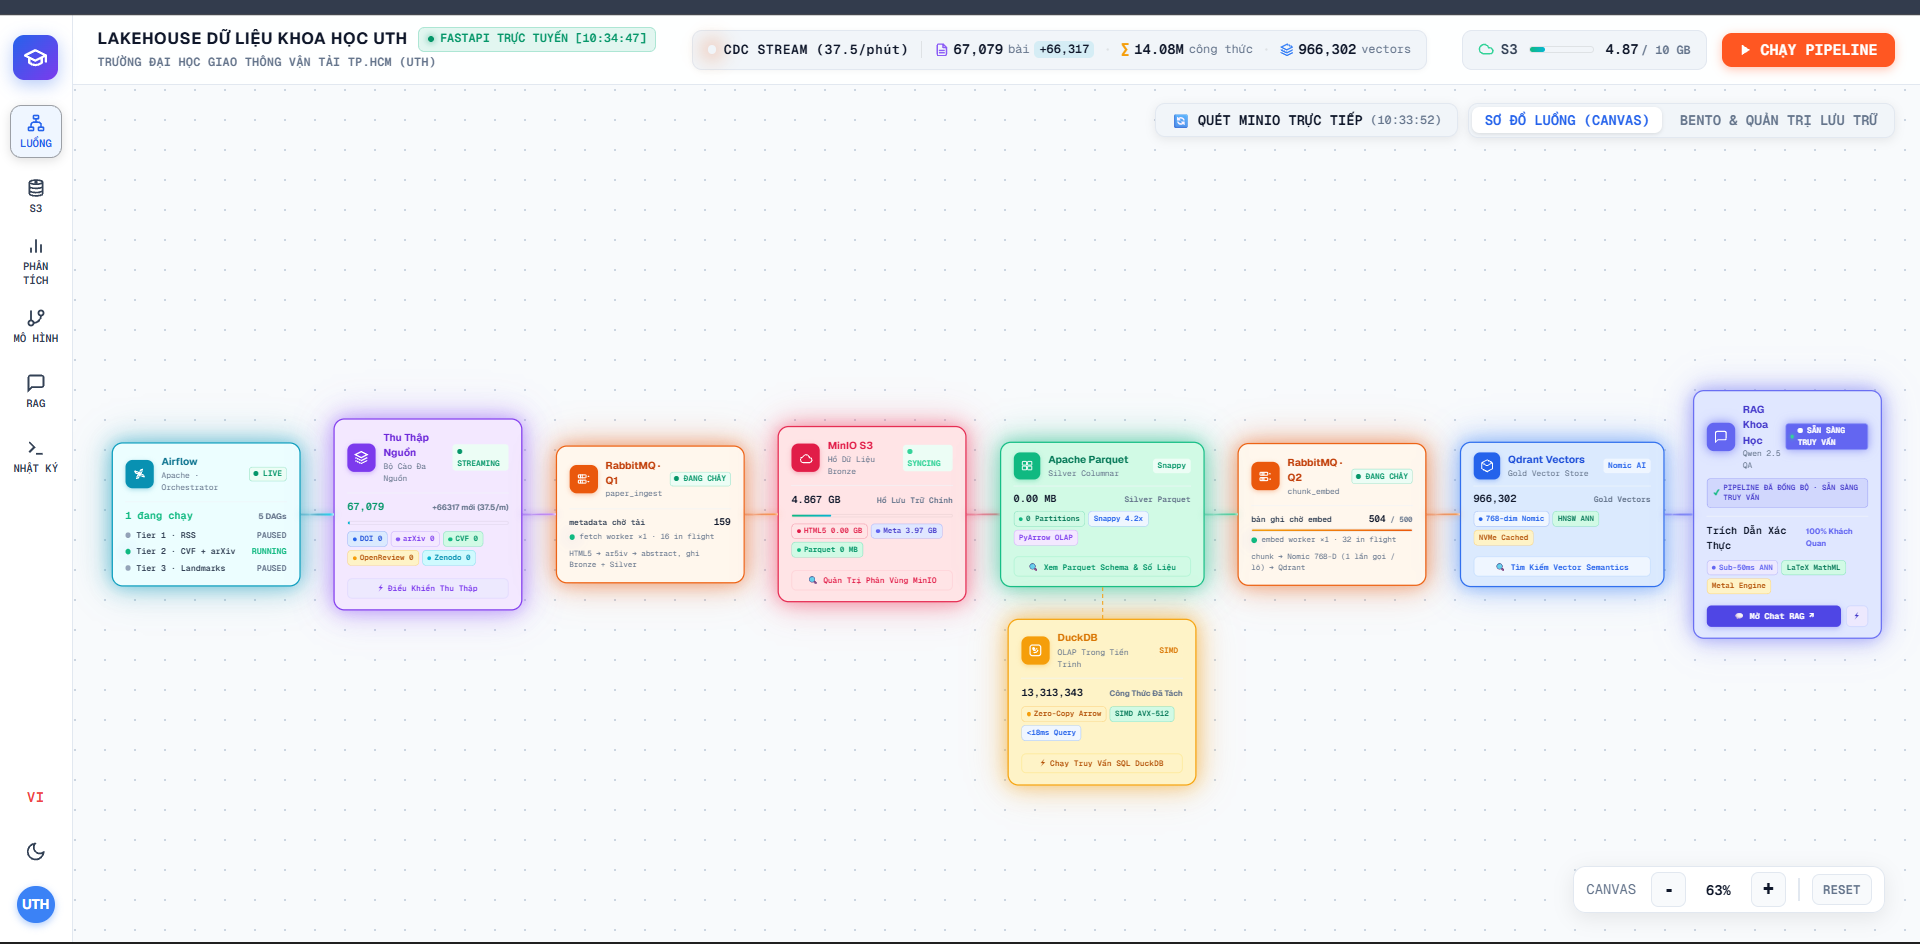
\includegraphics[width=\textwidth]{figures/lakehouse_canvas.png}
  \caption[Giao diện Lakehouse Canvas (ảnh tư liệu)]{Giao diện Lakehouse Canvas (ảnh tư liệu)}
  \ReportNote{Nguồn: ảnh lưu trong dự án LaTeX ngày 28/10/2026. Đây là giao diện của bản trước; số liệu trên ảnh không được dùng làm phép đo hiện tại.}
  \label{fig:lakehouse_canvas}
\end{figure}

\section{Phân Đoạn Ngữ Cảnh Chuyên Sâu (Domain-Aware Deep Chunking)}

Hiệu năng của hệ thống tìm kiếm vector RAG phụ thuộc trực tiếp vào chiến lược phân đoạn văn bản. Nếu cắt văn bản theo số ký tự cố định một cách cơ học (fixed-character chunking), một đoạn trích có thể bị cắt ngang giữa một công thức toán học hoặc mất hoàn toàn thông tin ngữ cảnh rằng đoạn đó thuộc về phần nào của bài báo.

Module \texttt{AcademicChunker} (triển khai tại \path{src/indexing/chunker.py}) thực thi chiến lược phân đoạn sâu theo ngữ cảnh:

\begin{enumerate}[label=\alph*)]
  \item \textbf{Abstract Chunk độc lập}: Tóm tắt của bài báo luôn được đóng gói thành một chunk riêng biệt có mã \texttt{\{paper\_id\}\_abs}. Đây là chunk có giá trị ngữ nghĩa đại diện cao nhất cho toàn bộ công trình.
  \item \textbf{Phân đoạn theo ranh giới mục}: Với section dài, cửa sổ tối đa 300 từ được cân bằng để hạn chế chunk đuôi ngắn. Overlap bằng 15\% độ dài cửa sổ, giới hạn 20--80 từ. Điểm bắt đầu/kết thúc ưu tiên ranh giới câu trong khoảng cho phép; đuôi dưới 40\% kích thước tối đa được gộp khi còn chỗ. Abstract vẫn là chunk độc lập, không áp dụng giới hạn 300 từ theo cùng cách với section dài.
  \item \textbf{Bổ sung ngữ cảnh nguồn (Contextual Enrichment)}: Mỗi đoạn trích sau khi cắt được tự động bổ sung tiêu đề bài báo và tên mục vào phần đầu:
  \begin{lstlisting}[language=Python]
context_text = f'Paper: "{title}" | Section: {sec_title}\n\n{chunk_text}'
  \end{lstlisting}
  Kỹ thuật này đảm bảo rằng khi một đoạn văn bản ngắn được nhúng thành vector, nó vẫn mang đầy đủ ngữ cảnh của bài báo chủ quản, ngăn chặn hiện tượng mất phương hướng ngữ nghĩa khi truy xuất độc lập.
\end{enumerate}

\section{Mô Hình Nhúng Vector Nomic Embed Text v1.5}

Hệ thống sử dụng mô hình nhúng mã nguồn mở \textbf{\path{nomic-ai/nomic-embed-text-v1.5}} với các đặc tính kỹ thuật vượt trội:
\begin{itemize}
  \item \textbf{Số chiều biểu diễn}: 768 chiều (768-D), là cấu hình vector của collection hiện tại; số chiều lớn hơn không tự chứng minh chất lượng cao hơn.
  \item \textbf{Hỗ trợ ngữ cảnh dài}: Khả năng xử lý lên tới \textbf{8,192 tokens} nhờ cấu trúc mã hóa vị trí quay (Rotary Position Embeddings - RoPE), cấu hình trong hệ thống giới hạn an toàn ở mức 2,048 tokens và có thể cắt bớt đầu vào dài vượt giới hạn.
  \item \textbf{Cơ chế tiền tố bất đối xứng (Asymmetric Task Prefixing)}: Mô hình được huấn luyện đặc thù cho bài toán truy xuất thông tin không đối xứng:
    \begin{itemize}
      \item Khi nhúng câu hỏi của người dùng: Thêm tiền tố \texttt{search\_query: <câu hỏi>}.
      \item Khi nhúng đoạn tài liệu học thuật: Thêm tiền tố \texttt{search\_document: <văn bản>}.
    \end{itemize}
  \item \textbf{Chuẩn hóa L2 (L2 Normalization)}: Toàn bộ vector đầu ra được chuẩn hóa $\|v\|_2 = 1$, biến phép tính khoảng cách Cosine thành tích vô hướng đơn giản: $\text{CosineSim}(u, v) = u \cdot v$, tối ưu hóa tốc độ tìm kiếm trên đồ thị HNSW của Qdrant.
\end{itemize}

\section{Luồng Hai Worker và Compaction}
Fetch nhận \texttt{scientific\_paper\_ingest}, kiểm tra trùng, lấy nội dung, ghi Bronze và part Silver papers rồi gửi bản ghi tới \texttt{scientific\_chunk\_embed}. Embed gom micro-batch, tạo chunk và vector, ghi part Silver chunks trước khi upsert Qdrant. Mỗi stage chỉ ACK khi đầu ra của stage đã bền vững; lỗi được thử lại trên hàng đợi của stage đó, quá số lần thử thì chuyển DLQ. Fetch tạm chờ khi hàng đợi embed đạt \texttt{EMBED\_QUEUE\_MAX}, mặc định 500.

DAG compact chạy mỗi 3 giờ, gộp parts của cả papers và chunks. Các part mới phát sinh trong khi compact được xử lý ở lần sau. Script migration/backfill có trong repository để hỗ trợ chuyển payload cũ sang Silver và bổ sung bài thiếu vector; chúng không được tự động chạy trong lần cập nhật báo cáo này.
